\section{Example}
\label{sec:example}

We next use an example to illustrate challenges in mining
API mapping relations. Figure~\ref{fig:challenge} shows a
Java code example and its translated C\# code. This Java code
example accepts a \CodeIn{string} input that represents the name of a
file or directory and returns a \CodeIn{boolean} value that
describes whether the file or directory exists. To achieve this functionality, the
code example declares a local variable, called \CodeIn{file}, of
type \CodeIn{java.io.File} and invokes the \CodeIn{exists} method. The
method takes the \CodeIn{string} input and \CodeIn{file} as its
inputs and produces the desirable \CodeIn{boolean} value. Here, we
consider \CodeIn{file} (a receiver) as a special input for
the \CodeIn{exists} method.

To translate this code example into C\#, a translation tool needs to
know mapping relations of API classes, so that it can translate inputs,
outputs, and variables into C\#. For example, the translation tool
needs to know the mapped API class in C\# for \CodeIn{java.io.File}
to translate the variable \CodeIn{file} to C\#. In addition, the
translation tool needs to know the mapped API methods, so that it can
add code for invoking proper API methods that take translated inputs and variables to
produce desirable outputs. For this example, the translation tool
adds code for invoking the \CodeIn{Exists} method and the
\CodeIn{FullName} method to achieve the functionality.
Here, we consider field accesses as special types of method invocations.

To mine these mapping relations, MAM uses projects such as Lucene
that have both Java and C\# versions. MAM includes three major steps
to mine the preceding two types of mapping relations of APIs from these projects.

\begin{figure}[t]
\begin{CodeOut}
\begin{alltt}
\textbf{Java code}:
1  File file = \textbf{new} File("test");
2  Boolean b = file.exists();
\textbf{Translated C\# code}:
3  FileInfo file = \textbf{new} FileInfo("test");
4  Boolean b = System.IO.File.Exists(file.FullName)||
           System.IO.Directory.Exists(file.FullName);
\end{alltt}
\end{CodeOut}\vspace*{-5ex}
\caption{\label{fig:challenge}Java code and its translated C\# code.}\vspace*{-2ex}
\end{figure}
\begin{figure}[t]
\begin{CodeOut}\vspace*{-1ex}
\begin{alltt}
\textbf{IndexFiles.java:}
5 public class IndexFiles \{
6   static final File INDEX_DIR = new File("index");
7   public static void main(String[] args) \{
      ...
8     if (INDEX_DIR.exists()) \{...\}
      ...
9       INDEX_DIR.delete(); \} \}
\textbf{IndexFiles.cs:}
10 class IndexFiles\{
11   internal static readonly System.IO.FileInfo INDEX_DIR
          = new System.IO.FileInfo("index");
12   public static void  Main(System.String[] args)\{
      ...
13     bool tmpBool;
14     if (System.IO.File.Exists(INDEX_DIR.FullName))
15       tmpBool = true;
16    else
17       tmpBool = System.IO.Directory
                         .Exists(INDEX_DIR.FullName);
      ... \} \}
\end{alltt}
\end{CodeOut}\vspace*{-4ex}
\caption{\label{fig:clientcode} Two versions (Java and C\#) of
client code.}\vspace*{-5ex}
\end{figure}

\textbf{Aligning client code.} First, MAM aligns classes and methods
between the two versions of each project. Since two code examples with
the same functionality of two languages may exhibit mapping
relations of APIs, this step aligns classes and methods by their
functionalities. To achieve this goal, MAM uses a mapping algorithm
based on similarities in the names of classes and methods defined
in the two versions of each project.

Aligning client code based on the names of classes and methods is based
on an observation on many existing projects such as
rasp\footnote{\url{http://sourceforge.net/projects/r-asp/}} are
migrated from one language to another. We observed that while
migrating the rasp project from C\# to Java, programmers first
renamed source files from C\# to Java and systematically addressed
the compilation errors by replacing C\# APIs with Java APIs. During
this procedure, the names of classes, methods, fields of classes, or
local variables in methods often remain the same or similar between
the two versions. Therefore, we use name similarities for aligning
client code of the two versions. For example, MAM aligns
\CodeIn{IndexFiles.java} with the \CodeIn{IndexFiles.cs} (shown in
Figure~\ref{fig:clientcode}) since the names of their classes and
methods are similar.
%\begin{figure}[t]
%\centering
%\includegraphics[scale=0.65,clip]{figure/dataflow.eps}\vspace*{-3ex}
% \caption
%{\label{fig:dataflow}API methods connected by inputs and
%outputs}\vspace*{-3ex}
%\end{figure}

\textbf{Mining API mapping of classes.} Next, MAM mines mapping
relations of API classes by comparing the names of data entities such as the names of
fields in aligned classes, variables, or parameters in aligned
methods. MAM uses name similarities for comparing the names of these
entities. For example, MAM identifies the \CodeIn{args} parameters in
Lines 7 (Java) and 12 (C\#) (Figure~\ref{fig:clientcode}) and maps
the API classes that are the types of the two parameters. Based on this
parameter, MAM maps the API class \CodeIn{java.lang.String} of Java
to \CodeIn{System.String} of C\#.

\textbf{Mining API mapping of methods.} After mapping API classes
between the two languages, MAM maps API methods. Mapping API methods
is challenging since often an API method of one language can be
mapped to multiple API methods of the other language. Furthermore,
mapping relations of API methods should also describe how parameters
and returns are mapped among these API methods. To address these challenges,
MAM constructs a graph, referred to as \emph{API Transformation
Graph} (ATG), for each aligned method of the client code in both
languages. These ATGs precisely capture inputs and outputs of API
methods, and help mine mapping relations of API methods.
For example, MAM mines a mapping relation from \CodeIn{java.io.File.Exists} in Java to 
\CodeIn{System.IO.File. Exists} and \CodeIn{System.IO.Directory.Exists} in C\#. 
By a close look at the API document for these API methods, we can find that the Java method can check whether a file or directory exists, and this functionality is fulfilled by two C\# API methods: \CodeIn{System.IO. File.Exists} for checking whether a file exists and \CodeIn{System.IO. Directory.Exists} for checking whether a directory exists. Section~\ref{sec:approach:mappingtypes} presents more details on how
we mine these mapping relations of API methods.

%\begin{figure}[t]
%\centering %\hfill
%\includegraphics[scale=0.95,clip]{figure/sample.eps}\vspace*{-3ex}
% \caption{\label{fig:example}API mapping}\vspace*{-4ex}
%\end{figure}

%Based on the mapping relations, a translation tool can migrate the
%preceding code snippet automatically. To learn the mapping
%relations,
%
%%\begin{figure}[t]
%%\centering
%%\includegraphics[scale=0.86,clip]{figure/openfile.eps}\vspace*{-1.5ex}
%% \caption
%%{\label{fig:openfile}Aligned client code}\vspace*{-2ex}
%%\end{figure}
%
%In this section, we illustrate the main steps of MAM to
%mine the API mapping in Java for \CodeIn{System.IO.Directory.
%Exists()} in C\# from the HypoLog
%project\footnote{\url{http://sourceforge.net/projects/twlog/}}.
%
%The first step of MAM is to align classes and methods of
%client code by names. This step finds class pairs and method pairs
%that implement similar functionalities, and each pair may use
%API mapping since it implements a similar functionality. Our
%approach chooses names to align classes and methods because these
%classes and methods are from the same project. In this example, our
%approach aligns the two methods as shown in
%Figure~\ref{fig:openfile} because the two method have similar names
%and their declaring classes also have similar names (see
%Section~\ref{sec:approach:alignclientcode} for details).
%
%The second step of MAM is to mine mapping relations of API
%classes based on the names of corresponding fields, parameters,
%returned types, and local variables. This step also relies on names
%for the same consideration of the first step. For example, our
%approach maps the two parameters with the same name as shown by the
%red arrow of Figure~\ref{fig:openfile}. From the types of the two
%parameters, MAM mines the mapping relation between two API
%classes: \CodeIn{System.String} $\leftrightarrow$
%\CodeIn{java.lang.String} (see
%Section~\ref{sec:approach:mappingtypes} for details).
%
%
%The final step of MAM is to mine mapping relations of API
%methods. Besides the factors listed in
%Section~\ref{sec:introduction}, another factor is that API calls in
%client code are often not carefully aligned. To deal with those
%challenges, MAM first builds an API Transformation Graph
%(ATG) for each method. After that, MAM compares built
%graphs to mine mapping relations of API methods (see
%Section~\ref{sec:approach:mappingtypes} and
%Figure~\ref{fig:approach1} for details). Figure~\ref{fig:example}
%shows the mined mapping relation between
%\CodeIn{System.IO.Directory.Exists()} and its API mapping in
%Java.
